\documentclass[usenatbib]{mn2e}
\usepackage{amsmath} 
\usepackage{amssymb} 
\usepackage{graphics}
\usepackage{graphicx}
\usepackage{epsfig}  
\usepackage{morefloats}
\def\be{\begin{equation}}
\def\ee{\end{equation}}
\def\ba{\begin{eqnarray}}
\def\ea{\end{eqnarray}}

\newcommand{\documentname}{paper~}
\newcommand{\match}{{\tt match}~}
\newcommand{\apj}{ApJ}  
\newcommand{\apjs}{ApJS}  
\newcommand{\apjl}{ApJL}  
\newcommand{\aj}{AJ}  
\newcommand{\mnras}{MNRAS}  
\newcommand{\mnrassub}{MNRAS accepted}  
\newcommand{\aap}{A\&A}  
\newcommand{\aaps}{A\&AS}  
\newcommand{\araa}{ARA\&A}  
\newcommand{\nat}{Nature}  
\newcommand{\physrep}{PhR}
\newcommand{\pasp}{PASP}    
\newcommand{\pasj}{PASJ}    

\newcommand{\kms}{\,km~s$^{-1}$}
\def\squig{\sim\!\!}
\newcommand{\LCDM}{$\Lambda$CDM~}
\newcommand{\beq}{\begin{eqnarray}}  
\newcommand{\eeq}{\end{eqnarray}}   
\newcommand{\zz}{$z\sim 3$} 
\newcommand{\avg}[1]{\langle{#1}\rangle}  
\newcommand{\ly}{{\ifmmode{{\rm Ly}\alpha}\else{Ly$\alpha$~}\fi}}
\newcommand{\hMpc}{{\ifmmode{h^{-1}{\rm Mpc}}\else{$h^{-1}$Mpc }\fi}}  
\newcommand{\hGpc}{{\ifmmode{h^{-1}{\rm Gpc}}\else{$h^{-1}$Gpc }\fi}}  
\newcommand{\hmpc}{{\ifmmode{h^{-1}{\rm Mpc}}\else{$h^{-1}$Mpc }\fi}}  
\newcommand{\hkpc}{{\ifmmode{h^{-1}{\rm kpc}}\else{$h^{-1}$kpc }\fi}}  
\newcommand{\hMsun}{{\ifmmode{h^{-1}{\rm
        {M_{\odot}}}}\else{$h^{-1}{\rm{M_{\odot}}}$}\fi}}   
\newcommand{\hmsun}{{\ifmmode{h^{-1}{\rm
        {M_{\odot}}}}\else{$h^{-1}{\rm{M_{\odot}}}$}\fi}}   
\newcommand{\Msun}{{\ifmmode{{\rm {M_{\odot}}}}\else{${\rm{M_{\odot}}}$}\fi}}  
\newcommand{\msun}{{\ifmmode{{\rm {M_{\odot}}}}\else{${\rm{M_{\odot}}}$}\fi}}  
\newcommand{\lya}{{Lyman$\alpha$~}}
\newcommand{\clara}{{\texttt{CLARA}}~}
\newcommand{\rand}{{\ifmmode{{\mathcal{R}}}\else{${\mathcal{R}}$ }\fi}}  
\newcommand{\Lsun}{\mbox{\,$L_{\odot}$}}
\newcommand{\like}{\mathscr{L}}
\newcommand{\bftheta}{\mathbf{\Theta}}
\newcommand{\degree}{\ensuremath{^\circ}}
\def\spose#1{\hbox to 0pt{#1\hss}}
\def\simlt{\mathrel{\spose{\lower 3pt\hbox{$\mathchar"218$}}
     \raise 2.0pt\hbox{$\mathchar"13C$}}}
\def\simgt{\mathrel{\spose{\lower 3pt\hbox{$\mathchar"218$}}
     \raise 2.0pt\hbox{$\mathchar"13E$}}}
\font\smcap=cmcsc10

\begin{document}

\title[Quasar line profiles from  rest-frame UV to Optical]{Quasar line profiles from rest-frame UV to Optical}    
\author[P. Lira and J.E. Mejia-Restrepo]{
\parbox[t]{\textwidth}{\raggedright 
Paulina Lira $^{1}$ and
Juli\'an Mej\'ia-Restrepo$^{1}$ 
}
\vspace*{6pt}\\
$^{1}$ Departamento de Astronom\'{i}a, Universidad de Chile, Camino el
Observatorio 1515, Santiago, Chile} 

\maketitle

\begin{abstract}
 Quasar line profiles from  rest-frame UV to Optical 
\end{abstract}

\begin{keywords}
{galaxies: AGNs, quasars, Broad line region} 
\end{keywords}


\section{Spectral Measurements}

\subsection{Continuum and Spectral Indices}

Our first approach to characterize the quasar continua consisted in using a single power law. ( $F_{\lambda} \propto \lambda^{\alpha}$ ) over the entire spectra wavelenght coverage (1200-9000$\AA$) of our sample. We have found that, in general, this single power-law does not give a good representation of the overall continua and we need  at least a composite of two power law with different slopes instead: a broken power law.
The last result motivates us to use accretion-thin-disk models (ADMs) to  characterize the quasar continua.  These model are not only a more physical approach but also has intrinsic continuum slope changes. We have  taken into account the effect of galactic extinction on the spectra before fitting the continuum model.




\subsection{Small Blue Bump}

The UV-optical continuum spectra of AGNs  show a bump between 2000 and 4000 $\AA$ which is known as the small blue bump (SBB). The SBB  consists  of unresolved Fe emission and Balmer continuum.  
The Balmer continuum is modeled  using a theoretical template provided by Hagai Netzer. We force such template to coincide in mean flux over the $3640-3650 \AA$ wavelength  region were the FeII emission is known to be weak (citation required). To include the effect of broadening on the high order lines of the balmer series we first fit the MgII line (as described below) and the we convolve its computed line width with the original balmer continuum (600km/s). It is important to emphazise that this convolution will affect thelines on balmer series but will have no effect bellow the balmer limit due to the functional flatness of this part of the model.



Meanwhile, the Fe emission is modeled  using the FeII and FeIII template of  Vestergaard \& Wilkes 2001 derived from the  1Zw 1 narrow-line quasar (900km/s). We allow the template to vary in both: intensity and broadening. 
This template has a a cut off around 3080$\AA$ that does not let us to model the Fe emission for wavelengths between 3080 and 4000 $\AA$. However, given that the MgII line center is around 2800 $\AA$ this cutoff does not affect the fitting of this line which is the most important in the small blue bump region. 




	
\subsection{Emission Lines}

 We take a global continuum as the baseline for all the lines in the spectrum.This global continuum is composed by the  accretion- disk-model continuum  and the Balmer continuum model. Both are subtracted before proceeding with the emission line fitting. For our line fitting procedure we do not consider any additional local continuum for any emission line. 



\subsubsection{General procedure}
For each of several emission-line regions we fit the emission line components using $\chi^2$ minimization with the package pyspeckit (Ginsburg et al 2011).
\\
We used a narrow ($500<=V(km/s)<=3000$) and a broad ($3000<=V(km/s)<=10000$) Gsaussian component to fit each strong, broad emission line. A velocity shift is allowed between the two components to account for the asymmetry of the line profile.
\\

 We have also restricted the velocity offset of those weak lines to hace a maximum of 1000km/s. I have given to the strong lines a maximum velocity offset of 4000km/s. The line centers of the lines of the same species are tied together but it is not the case for lines different of different atoms or ionization degree. 

Do you have any suggestion to reduce the parameter space.

For Halpha and Hbeta, we have also included a third Gaussian component to account for the  narrow-line region (NLR) emission on top of the broad-line profile. For weak emission lines only  one Gaussian component is used.
We used symmetric Gaussian profiles, so each profile has three parameters: flux, width, and central wavelength. We assume the same width for similar components of the same species, tie together the wavelengths of some lines based on their laboratory wavelengths, and assume line-intensity ratios for some lines based on their statistical weights  to avoid too many free parameters. We list in the appended table  all the free and dependent parameters in each region and how the parameters are related. 

When we find obvious strong absorption around a emission line of interest we exclude the absorbed regions before fitting. 



\subsubsection{MgII and H beta}

The MgII and H beta profile are fitted along with with the FeII templates of Vestergaard \& Wilkes 2001  and Boroson \& Green 1992 respectively.

Attached figures  show examples of our fitting results and individual components in each region of the J0019-
1053 quasar. We also show zooms in the balmer continuum, the en of the balmer series, an the FeII model close to MgII. 
Comments are detailed on the labels.

We can observe from these plots that in general we obtain good fits to the lines components using the constraints defined in the attached table. However, SiIV-OIV complex is not well reproduced by our gaussian models.   The main reason for this discrepancy is that our acreation disc model does not reproduce completely well the bluer part of this spectrum and it is sligthly below the real continuum. This leads the fitting code to interprete  this "overflux" as an additional gaussian component. (still working on a succesful Hbeta model because of some problems with the optical Fe template)


\begin{figure*}
\begin{center}
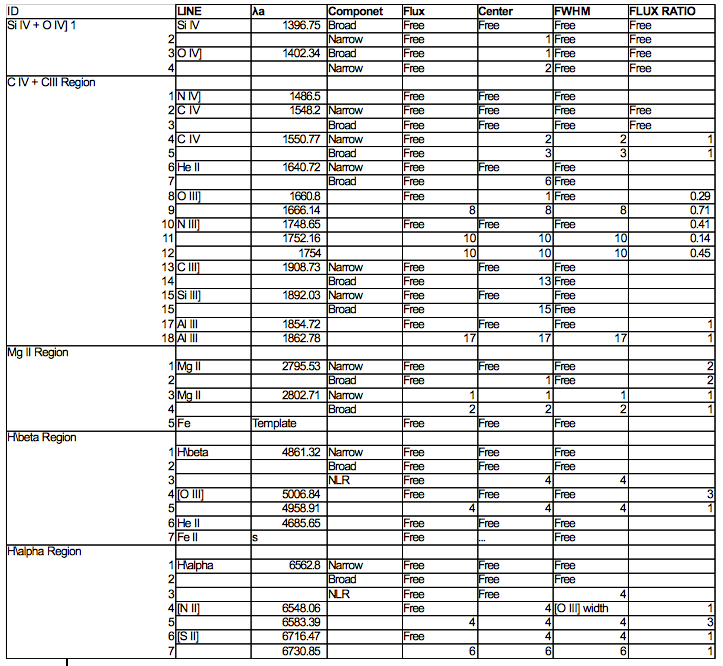
\includegraphics[width=0.7\linewidth,angle=0]{tab.png}
\vspace{5mm}
\end{center} 
\caption{Parameter definition \label{fig:landscape}}   
\end{figure*}
 
 \newpage

\section{Plots}

\subsection{Superposition}

\begin{figure*}
\begin{center}
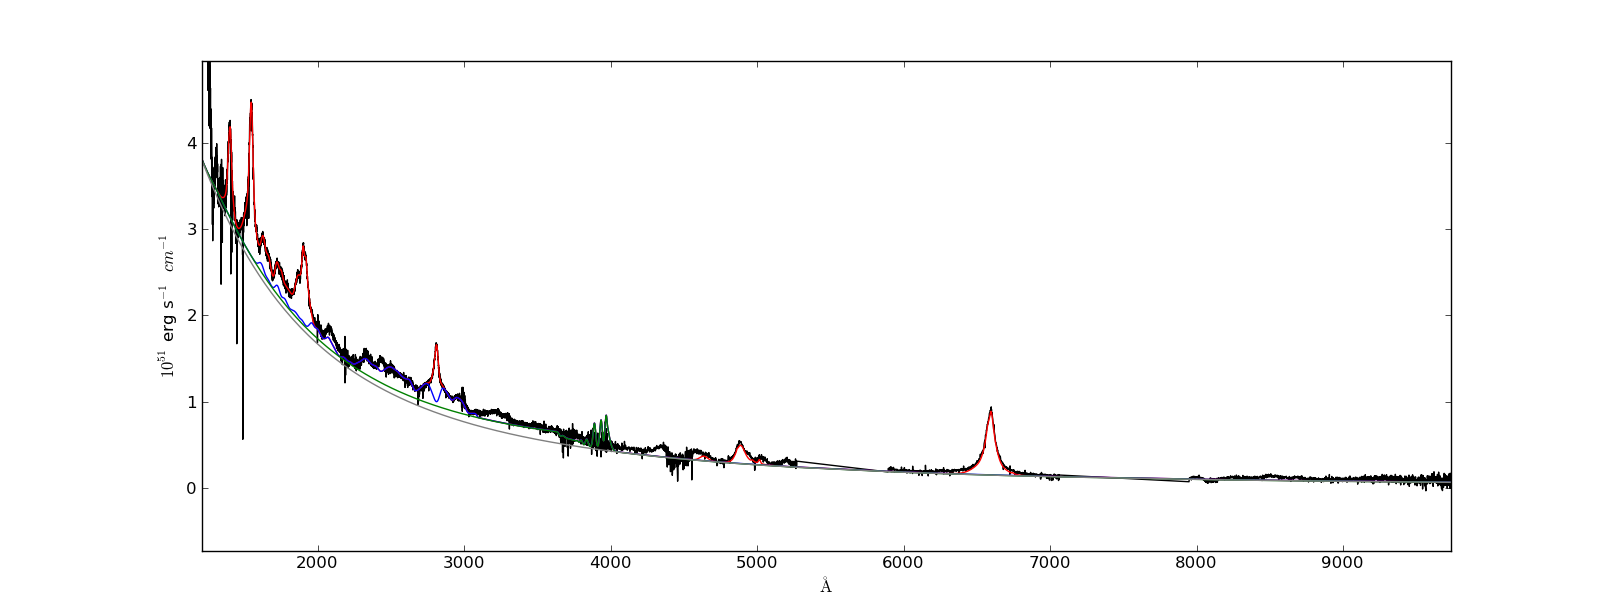
\includegraphics[width=0.6\linewidth,angle=0]{superposition_1.png}
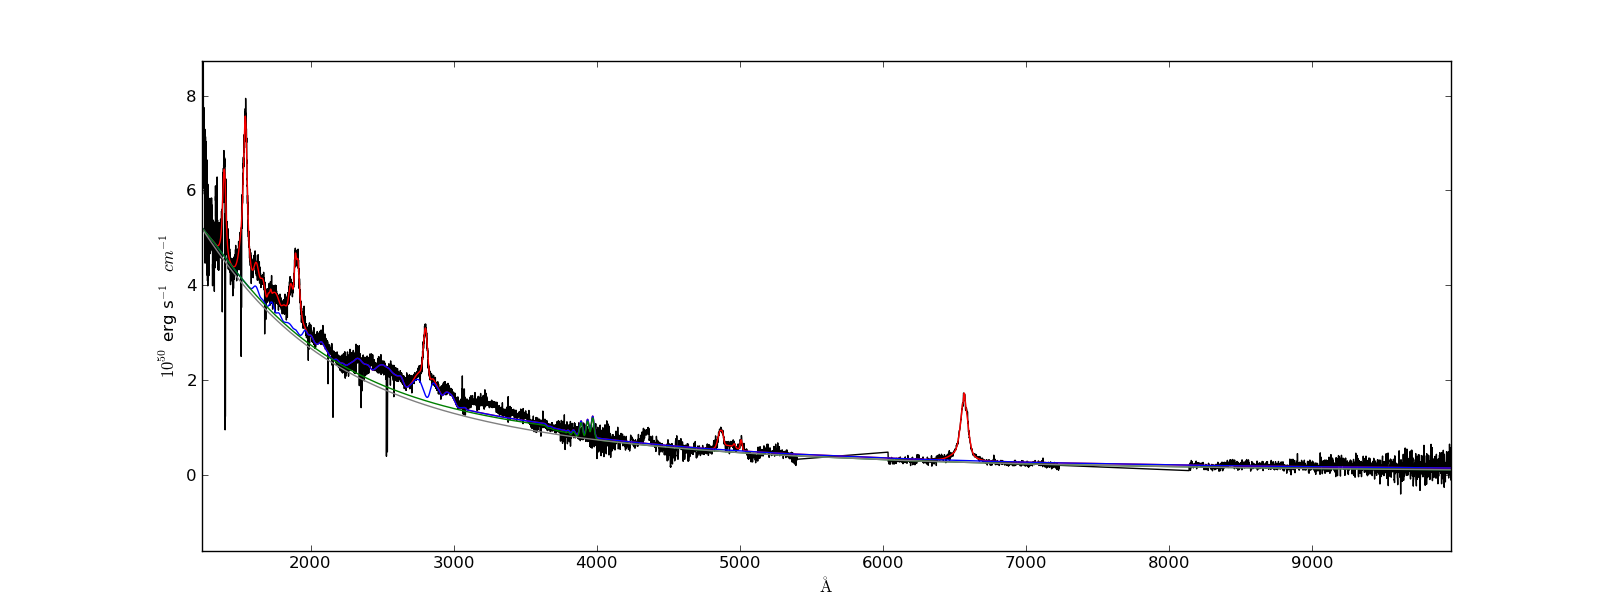
\includegraphics[width=0.6\linewidth,angle=0]{superposition_17.png}\\
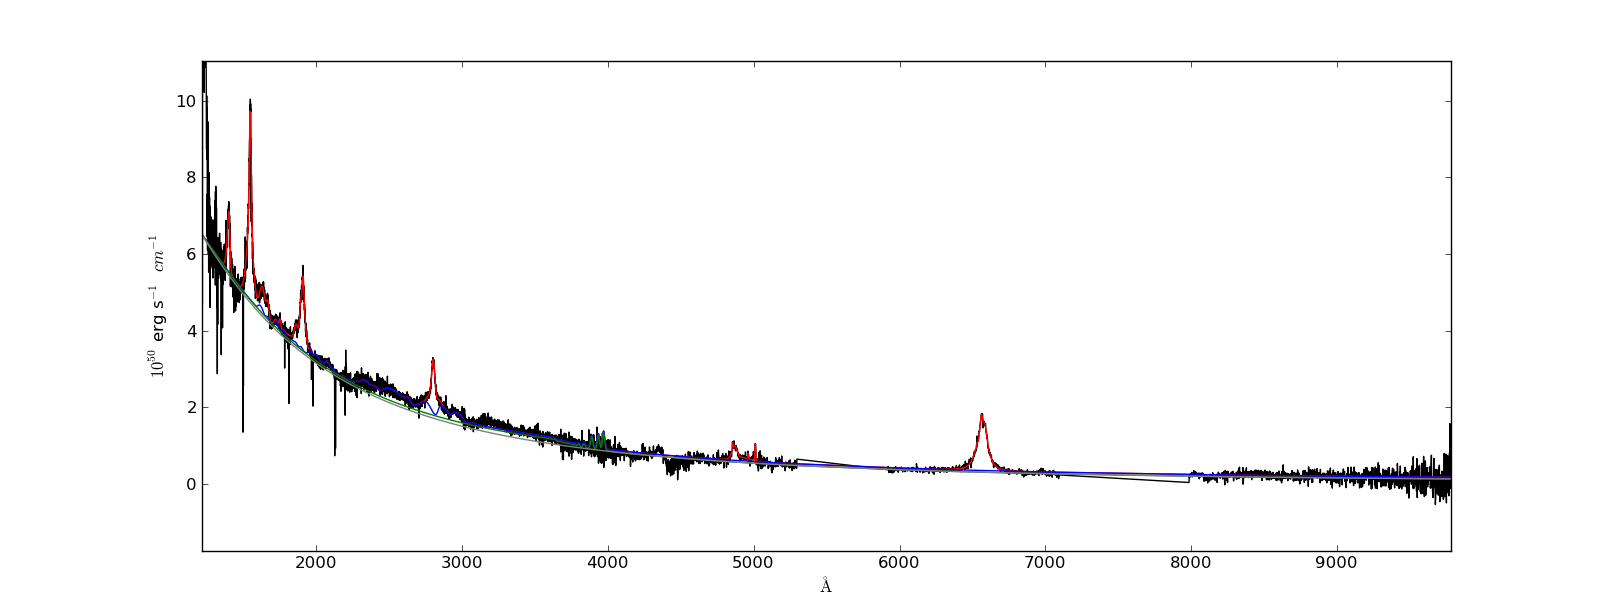
\includegraphics[width=0.6\linewidth,angle=0]{superposition_20.png}
\end{center} 
\caption{  Complete Spectra models.  Gray: continuum model, Green: Balmer + continuum, Blue: fe model + Balmer + continuum, Red: lines models + fe model + Balmer + continuum.  top: J0155-1023 (Group A) middle: J0136-0015 (GROUP E) bottom: J0223-0007 (GROUP E)     \label{fig:landscape}}   
\end{figure*}

\newpage

\subsection{Zoom 2000-4000A}

\begin{figure*}
\begin{center}
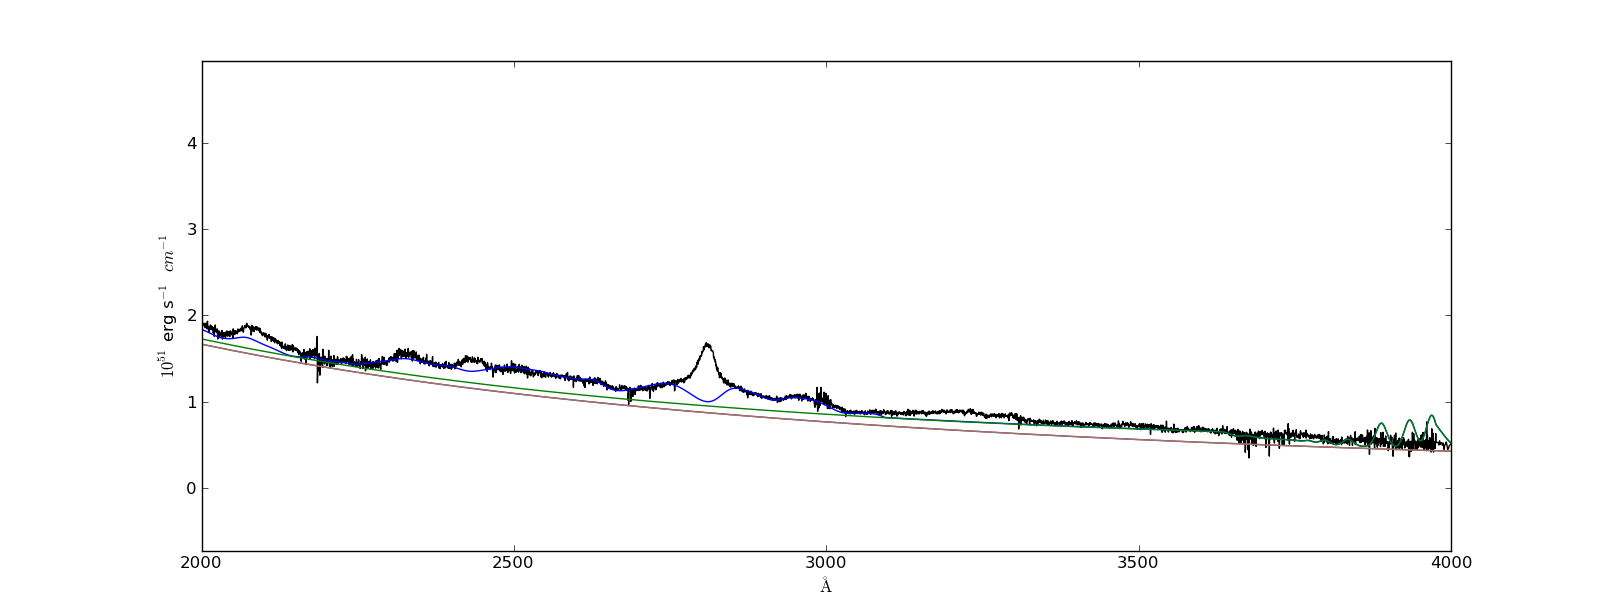
\includegraphics[width=0.6\linewidth,angle=0]{mg+fe_1.png}
\vspace{5mm}
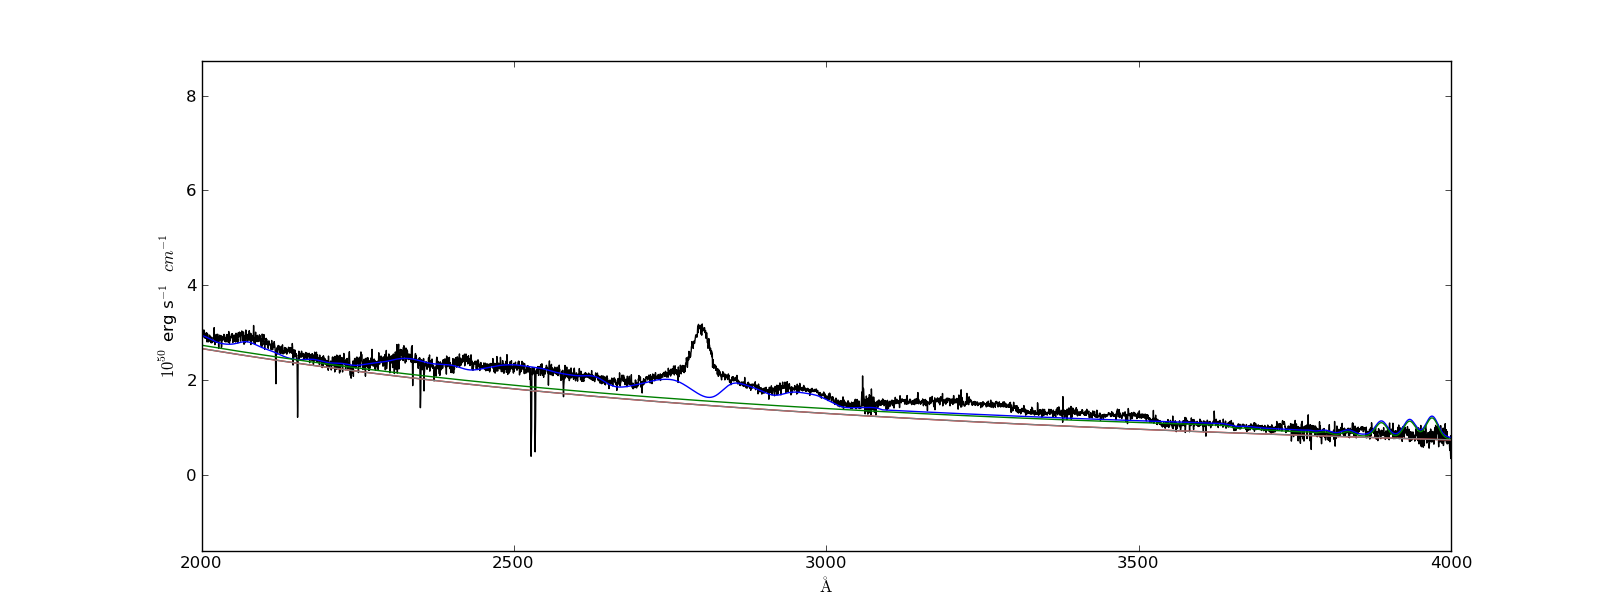
\includegraphics[width=0.6\linewidth,angle=0]{mg+fe_17.png}\\
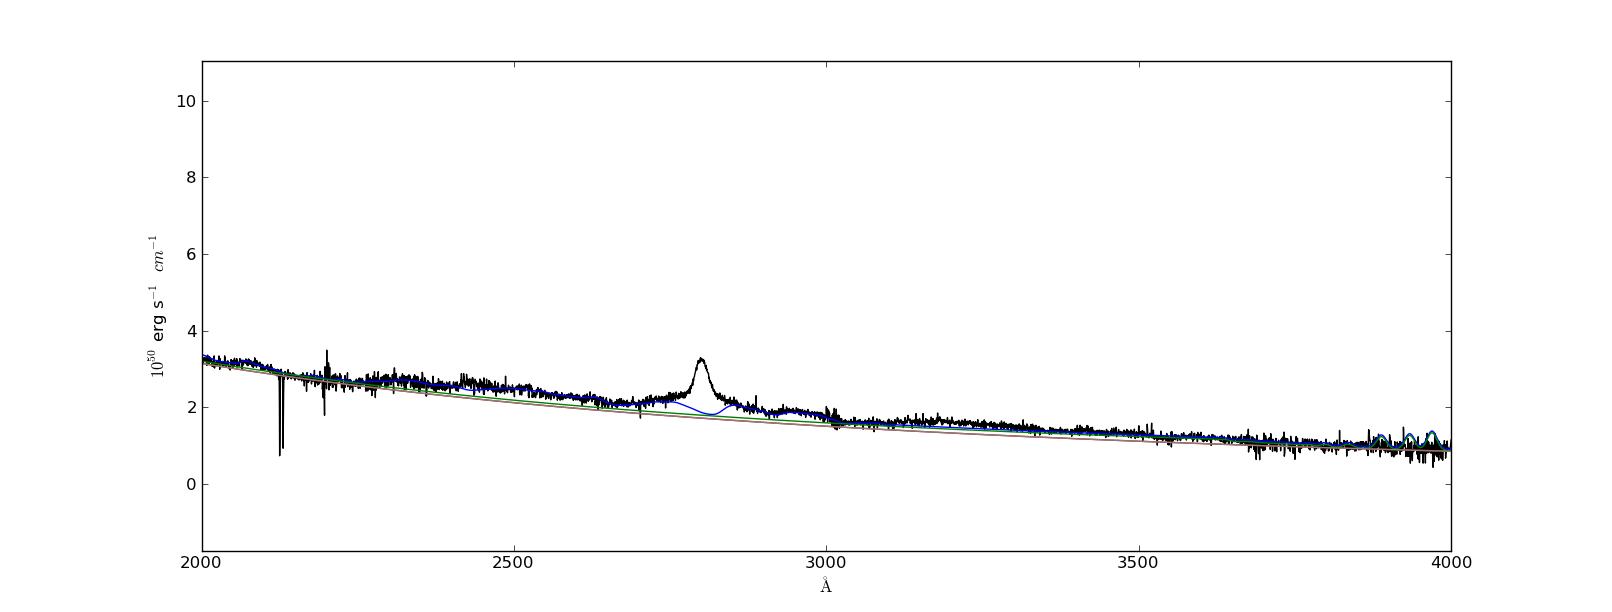
\includegraphics[width=0.6\linewidth,angle=0]{mg+fe_20.png}
\end{center} 
\caption{Zoom  on the small blue bump   top: J0155-1023 (Group A) middle: J0136-0015 (GROUP E) bottom: J0223-0007 (GROUP E) \label{fig:landscape}}   
\end{figure*}

\newpage

\subsection{Balmer lines}

\begin{figure*}
\begin{center}
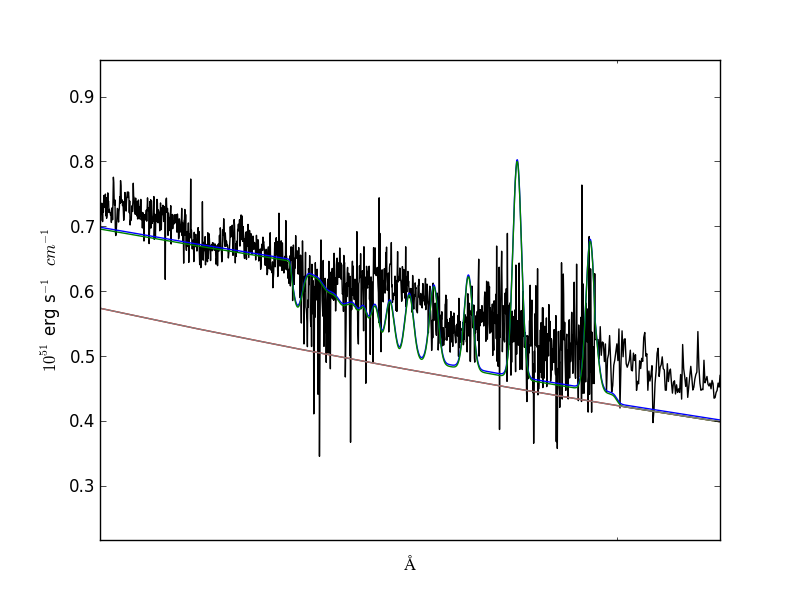
\includegraphics[width=0.6\linewidth,angle=0]{balmer_lines_1.png}
\vspace{5mm}
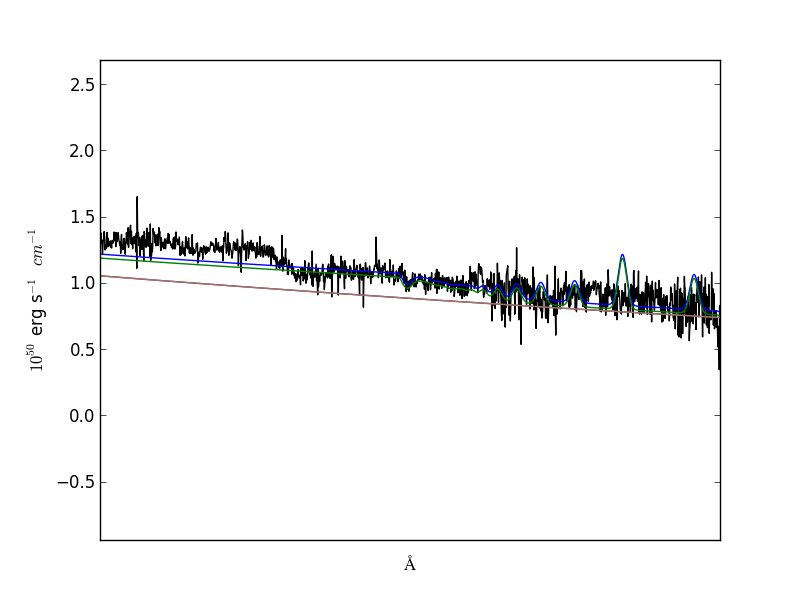
\includegraphics[width=0.6\linewidth,angle=0]{balmer_lines_17.png}\\
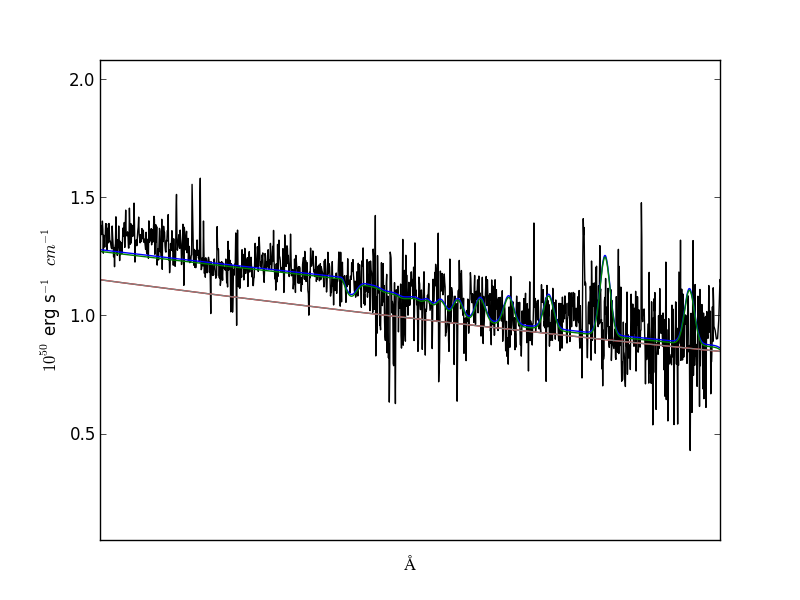
\includegraphics[width=0.6\linewidth,angle=0]{balmer_lines_20.png}
\end{center} 
\caption{Zoom on the balmer lines 3500-4000A (Transitions involving  the leves from 20 until 7 (3835A) ).   top: J0155-1023 (Group A) middle: J0136-0015 (GROUP E) bottom: J0223-0007 (GROUP E). It has a softer break after 3646A but still present.   \label{fig:landscape}}   
\end{figure*}

\newpage


\subsection{Zoom 2000-3100A}

\begin{figure*}
\begin{center}
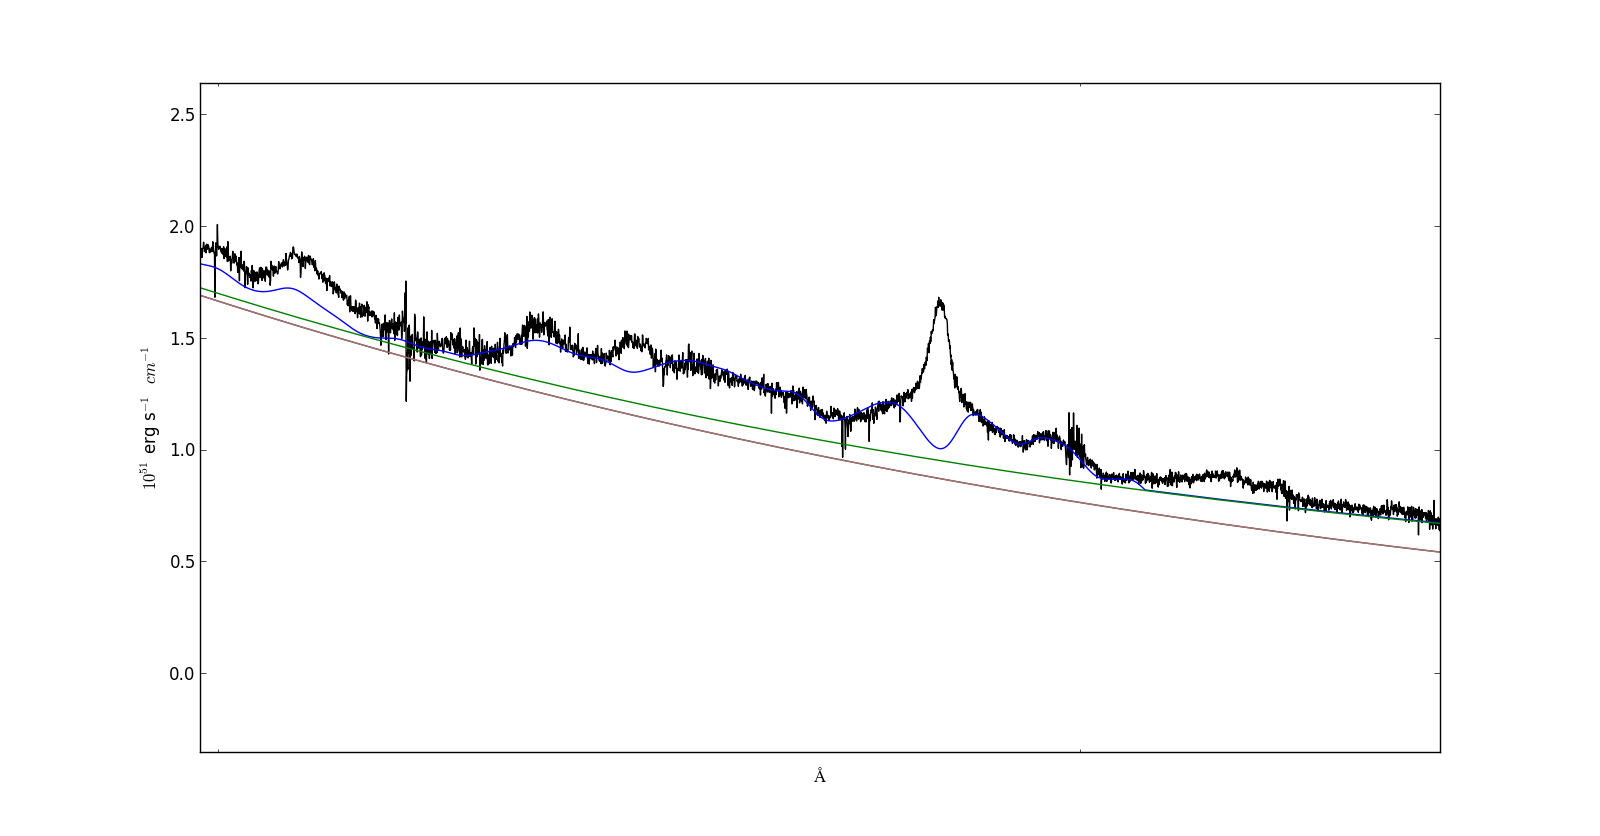
\includegraphics[width=0.6\linewidth,angle=0]{fe_2000-2800_1.png}
\vspace{5mm}
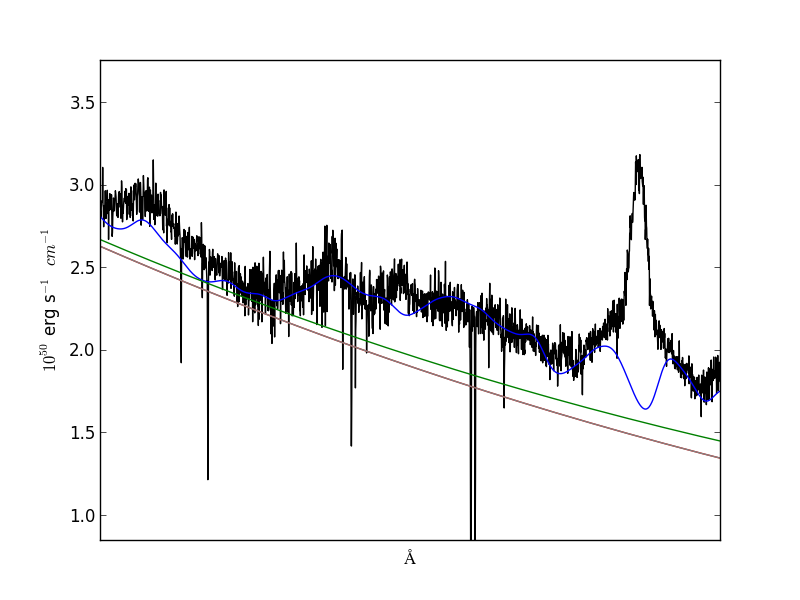
\includegraphics[width=0.6\linewidth,angle=0]{fe_2000-2800_17.png}\\
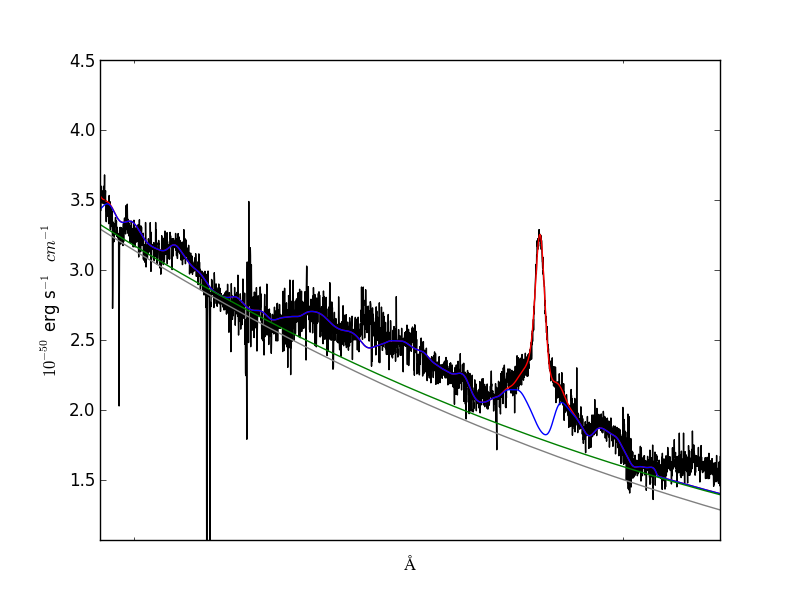
\includegraphics[width=0.6\linewidth,angle=0]{fe_2000-2800_20.png}
\end{center} 
\caption{Zoom on the FeII model. 3500-4000A (Transitions involving  the leves from 20 until 7 (3835A) ).   top: J0155-1023 (Group A) middle: J0136-0015 (GROUP E) bottom: J0223-0007 (GROUP E). In two of the spectra  we can see that below aprox 2200A the Fe model seems to be below the observed spectra maybe  because in those case a balmer continuum model with different tempareture is needed or could be the effect of   intrinsic extintion in the template. \label{fig:landscape}}   
\end{figure*}

\newpage

\subsection{MgII}

\begin{figure*}
\begin{center}
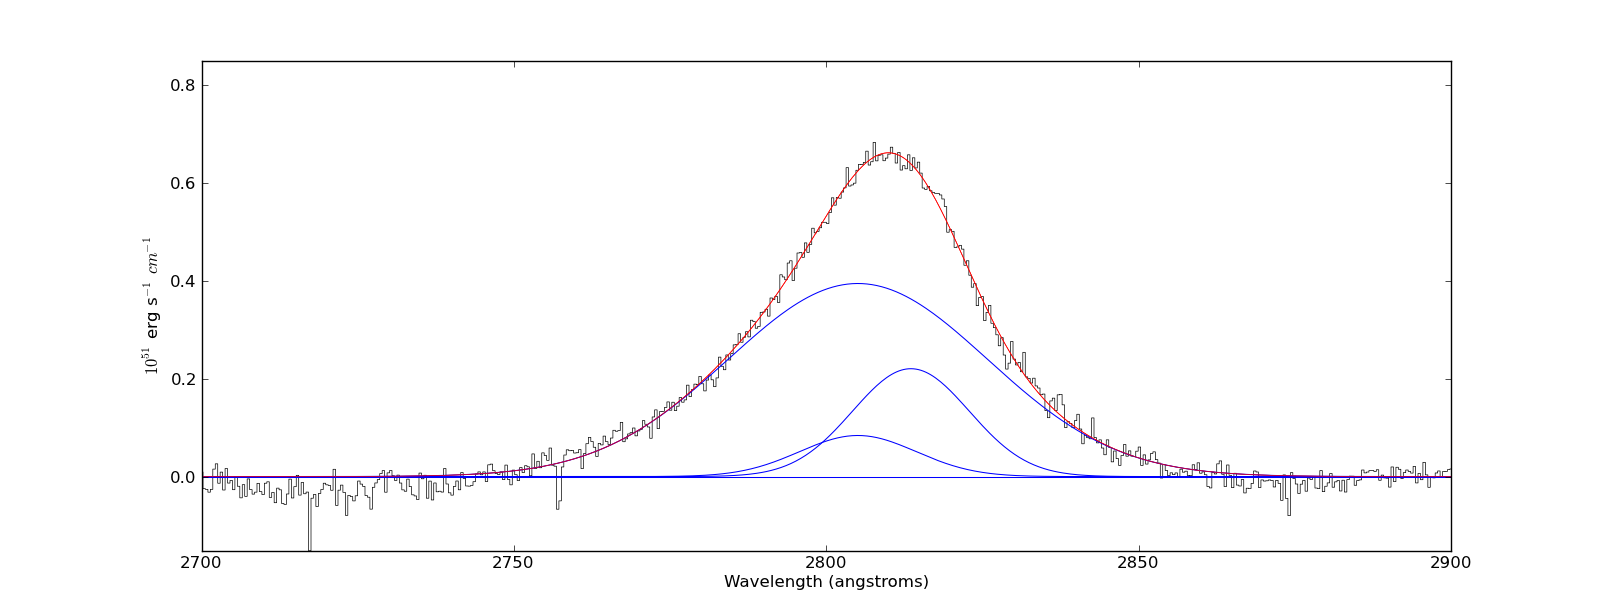
\includegraphics[width=0.46\linewidth,angle=0]{MgII_1.png}
\vspace{5mm}
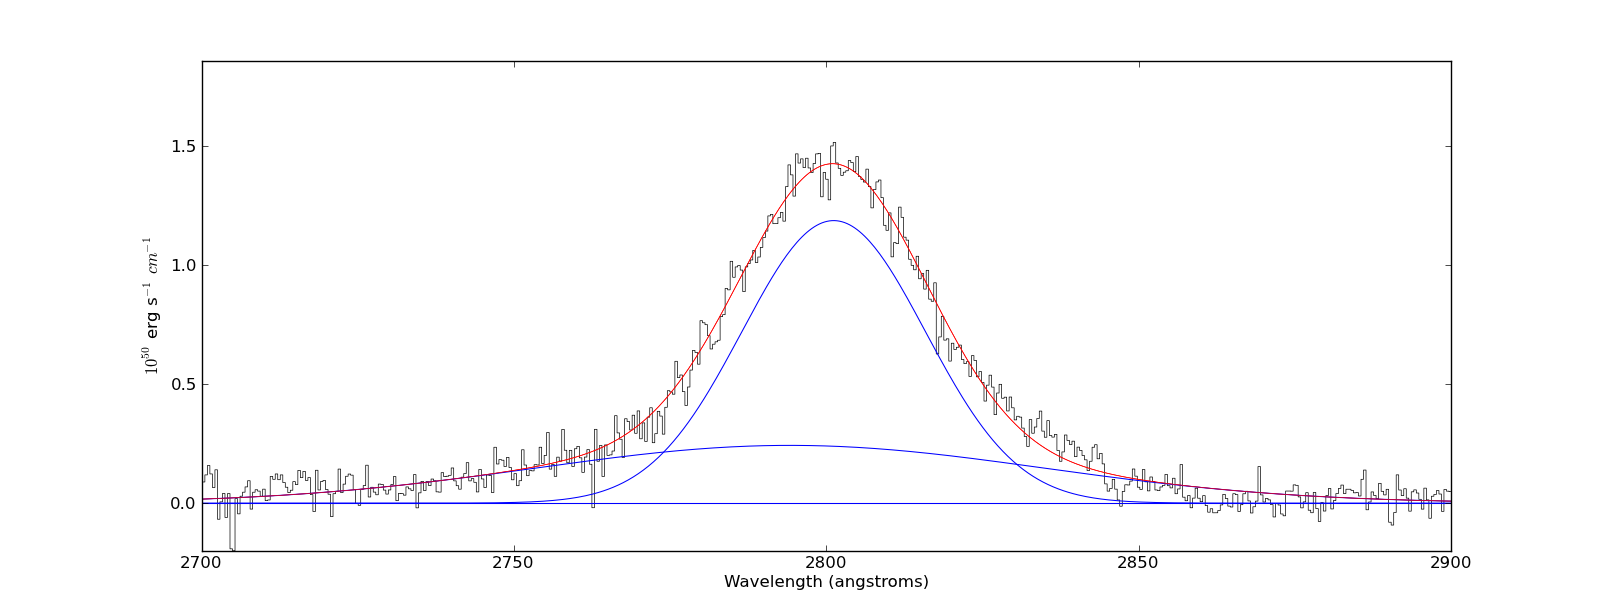
\includegraphics[width=0.49\linewidth,angle=0]{MgII_17.png}\\
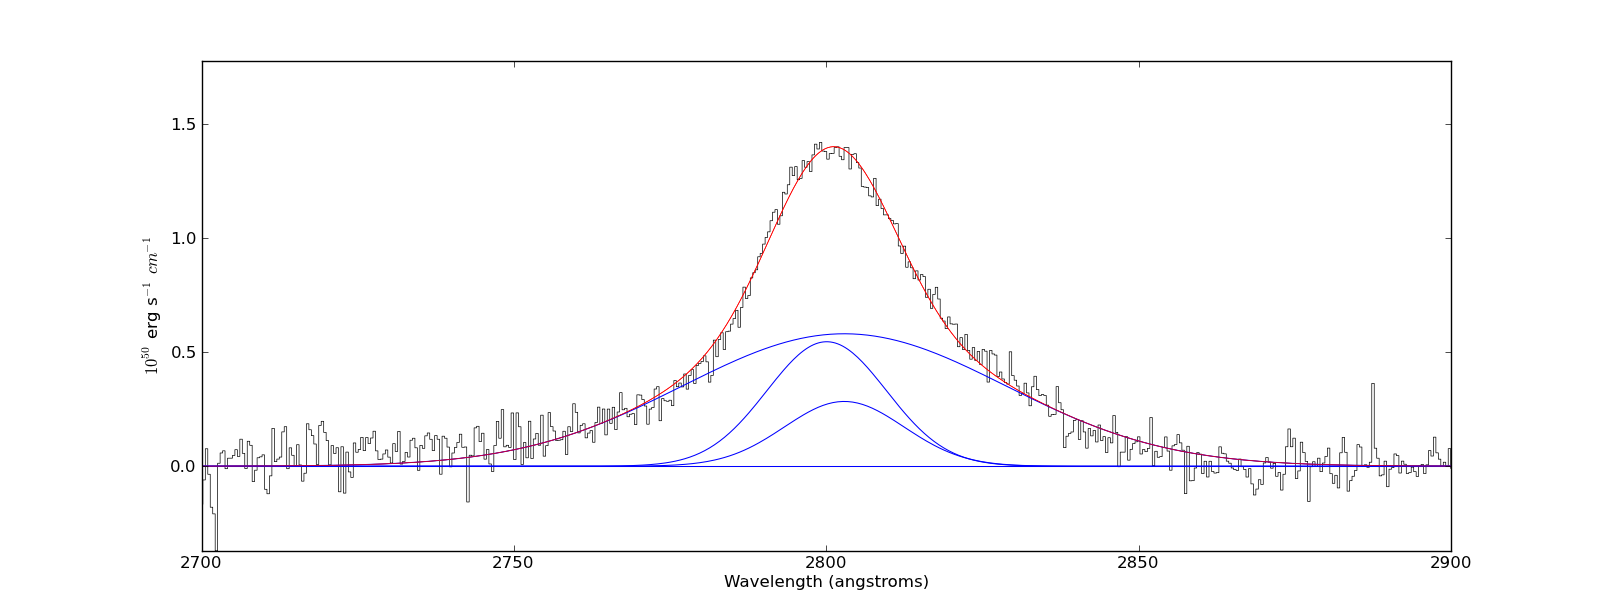
\includegraphics[width=0.46\linewidth,angle=0]{MgII_20.png}
\end{center} 
\caption{MgII. 3500-4000A (Transitions involving  the leves from 20 until 7 (3835A) ).   top: J0155-1023 (Group A) middle: J0136-0015 (GROUP E) bottom: J0223-0007 (GROUP E). \label{fig:landscape}}   
\end{figure*}

\newpage

\subsection{SiOIV}




\begin{figure*}
\begin{center}
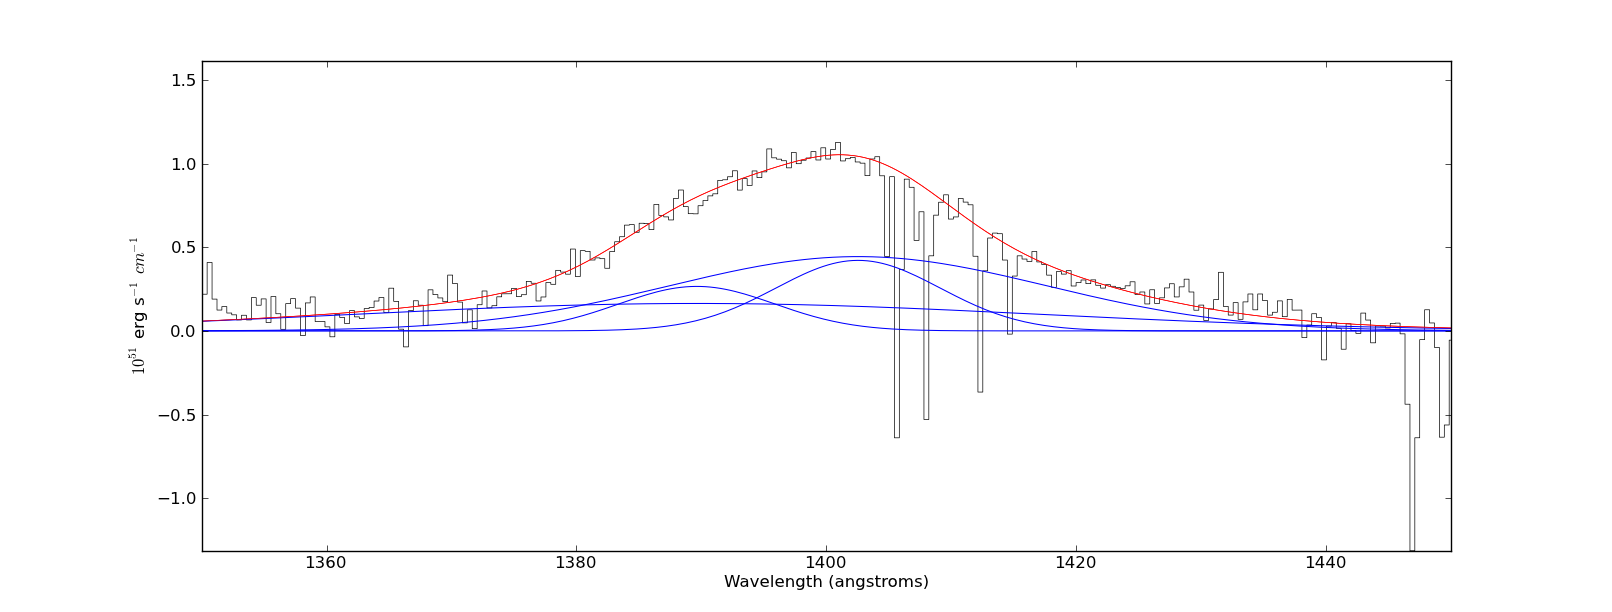
\includegraphics[width=0.46\linewidth,angle=0]{SiIV_1.png}
\vspace{5mm}
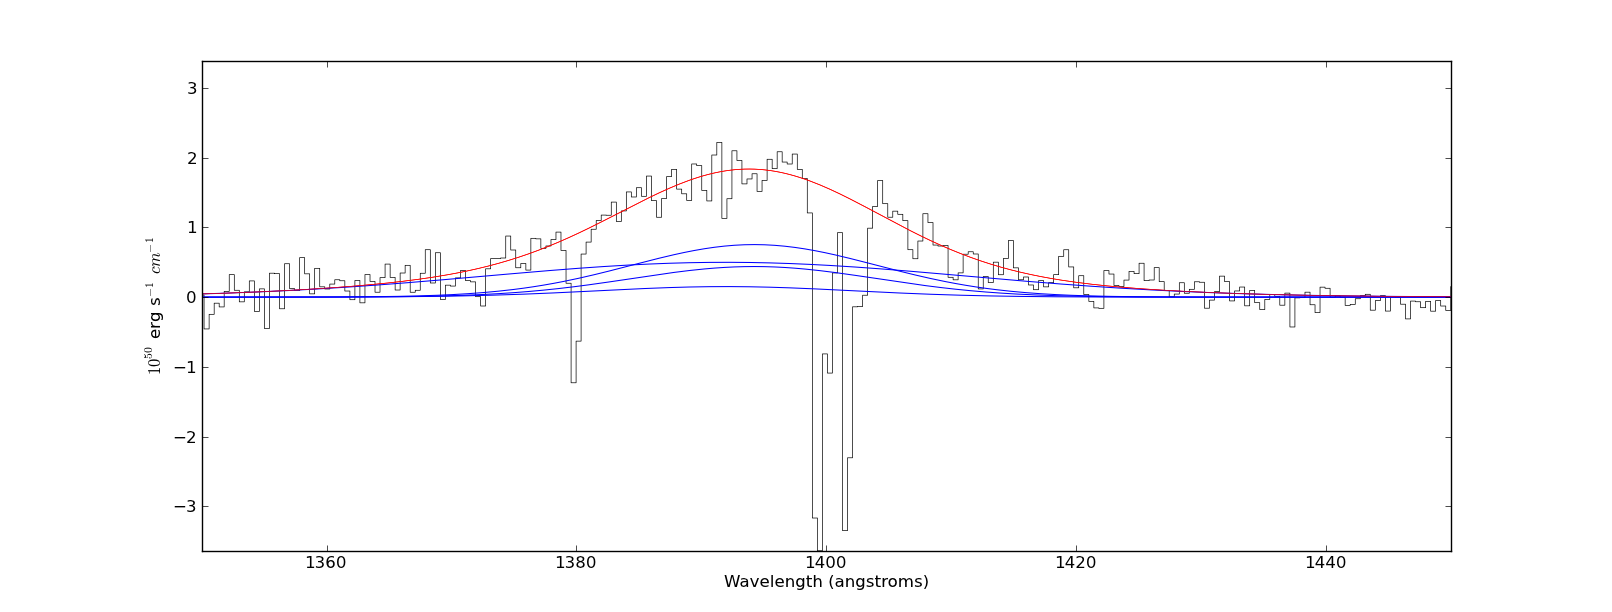
\includegraphics[width=0.49\linewidth,angle=0]{SiIV_17.png}\\
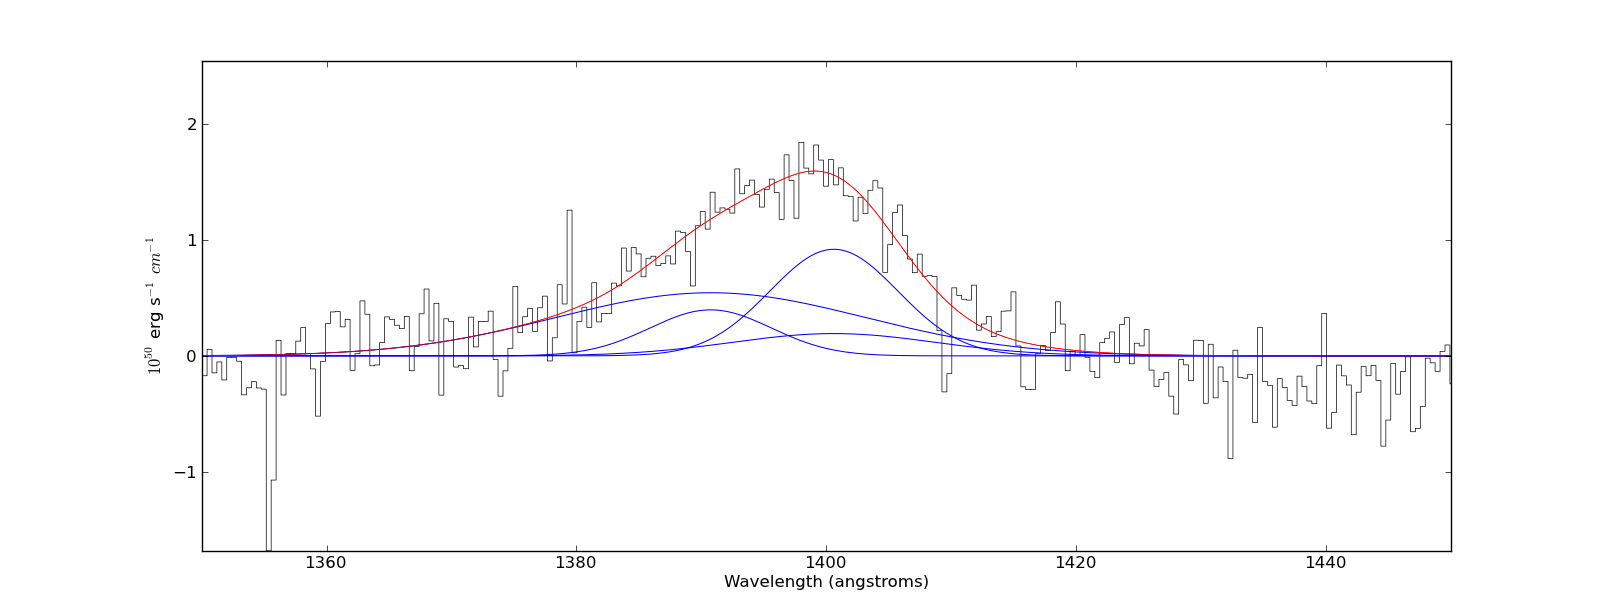
\includegraphics[width=0.46\linewidth,angle=0]{SiIV_20.png}
\end{center} 
\caption{SiIV+OIV Complex. 3500-4000A (Transitions involving  the leves from 20 until 7 (3835A) ).   top: J0155-1023 (Group A) middle: J0136-0015 (GROUP E) bottom: J0223-0007 (GROUP E) \label{fig:landscape}}   
\end{figure*}

\newpage







\subsection{CIV-CIII}

\begin{figure*}
\begin{center}
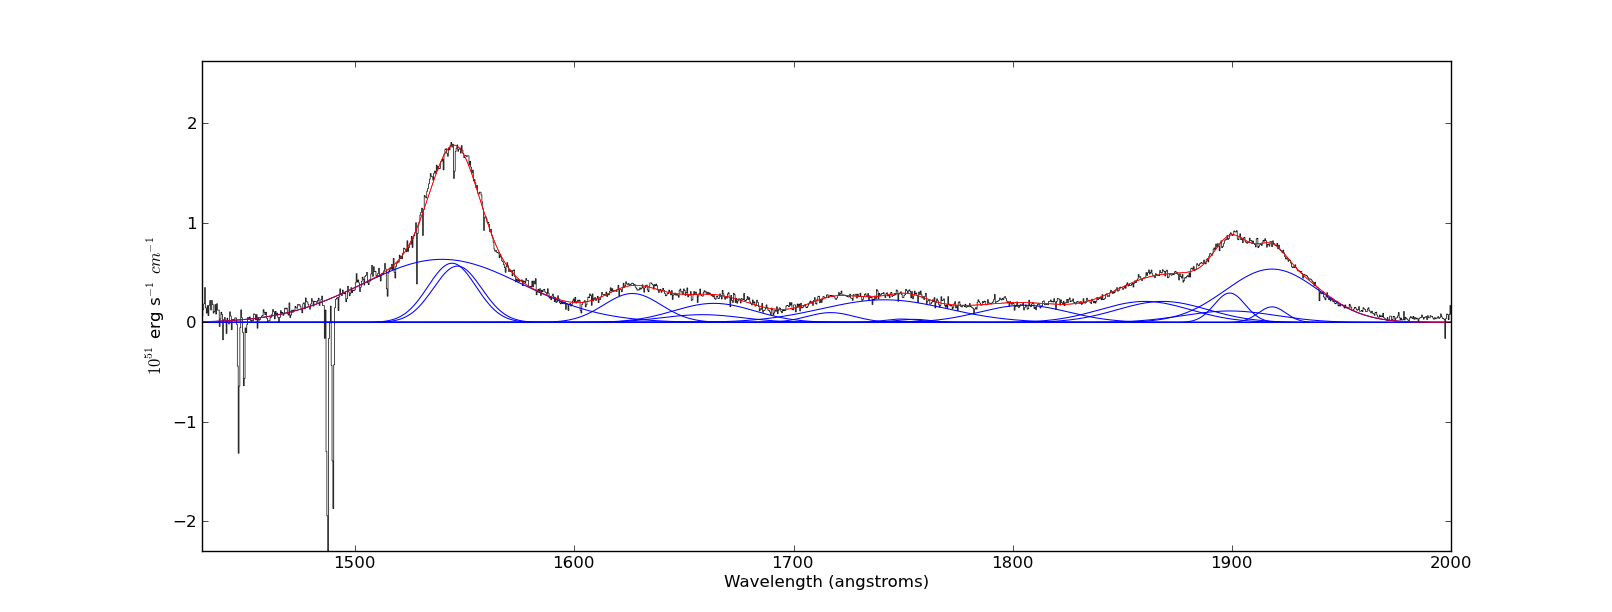
\includegraphics[width=0.46\linewidth,angle=0]{C_1.png}
\vspace{5mm}
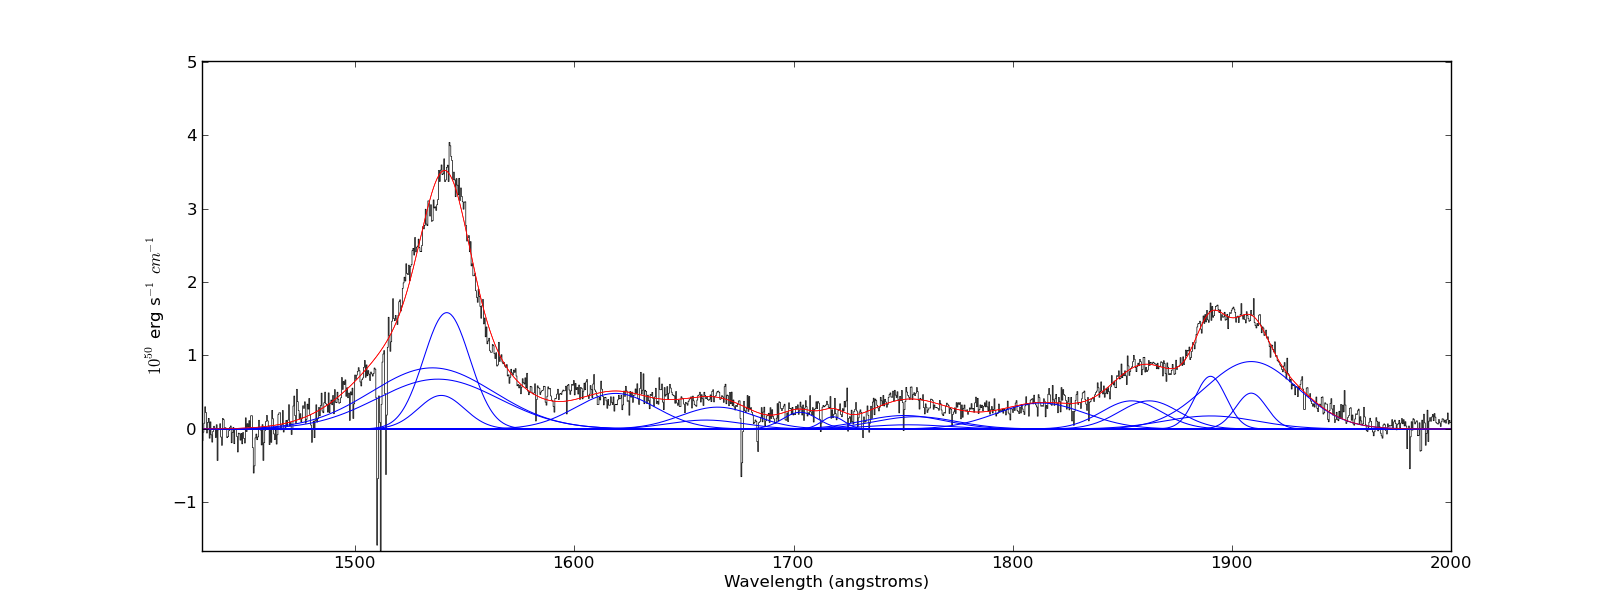
\includegraphics[width=0.49\linewidth,angle=0]{C_17.png}\\
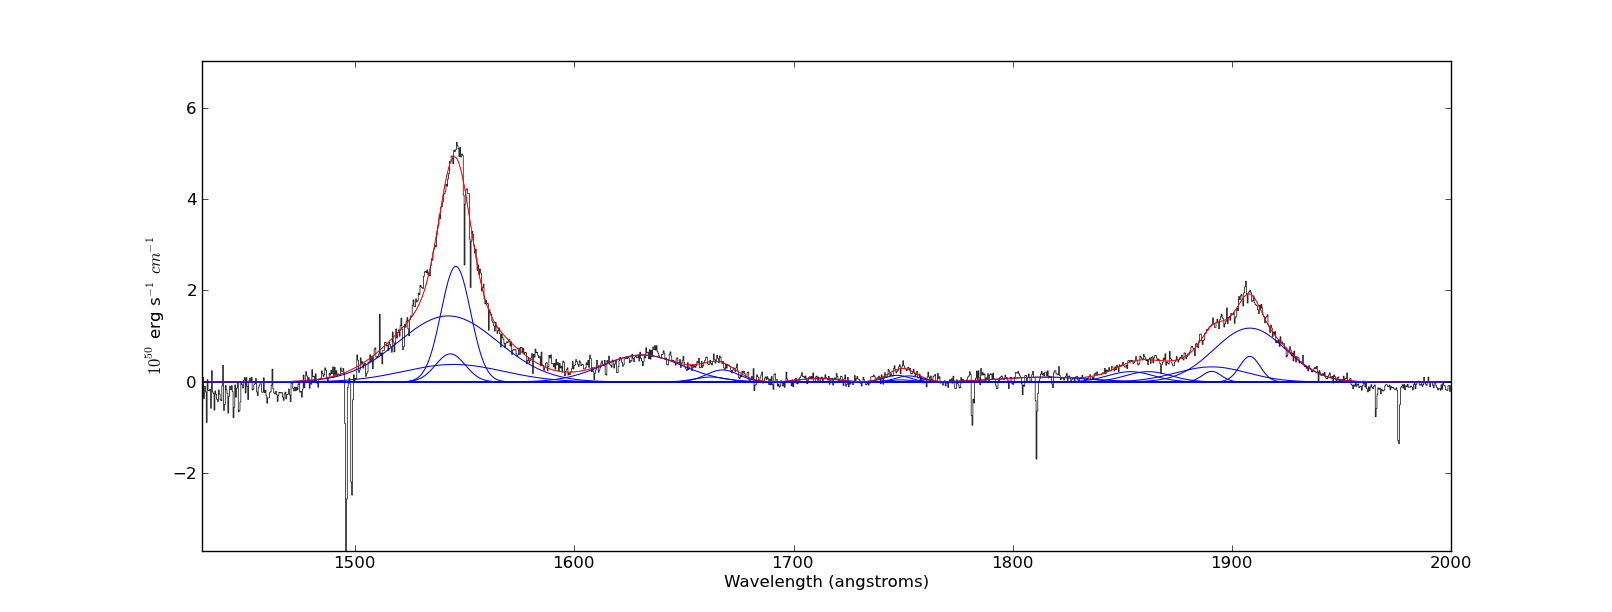
\includegraphics[width=0.46\linewidth,angle=0]{C_20.png}
\end{center} 
\caption{CIV +CIII Complex. 3500-4000A (Transitions involving  the leves from 20 until 7 (3835A) ).   top: J0155-1023 (Group A) middle: J0136-0015 (GROUP E) bottom: J0223-0007 (GROUP E) \label{fig:landscape}}   
\end{figure*}




\newpage

\subsection{H-$\alpha$}

\begin{figure*}
\begin{center}
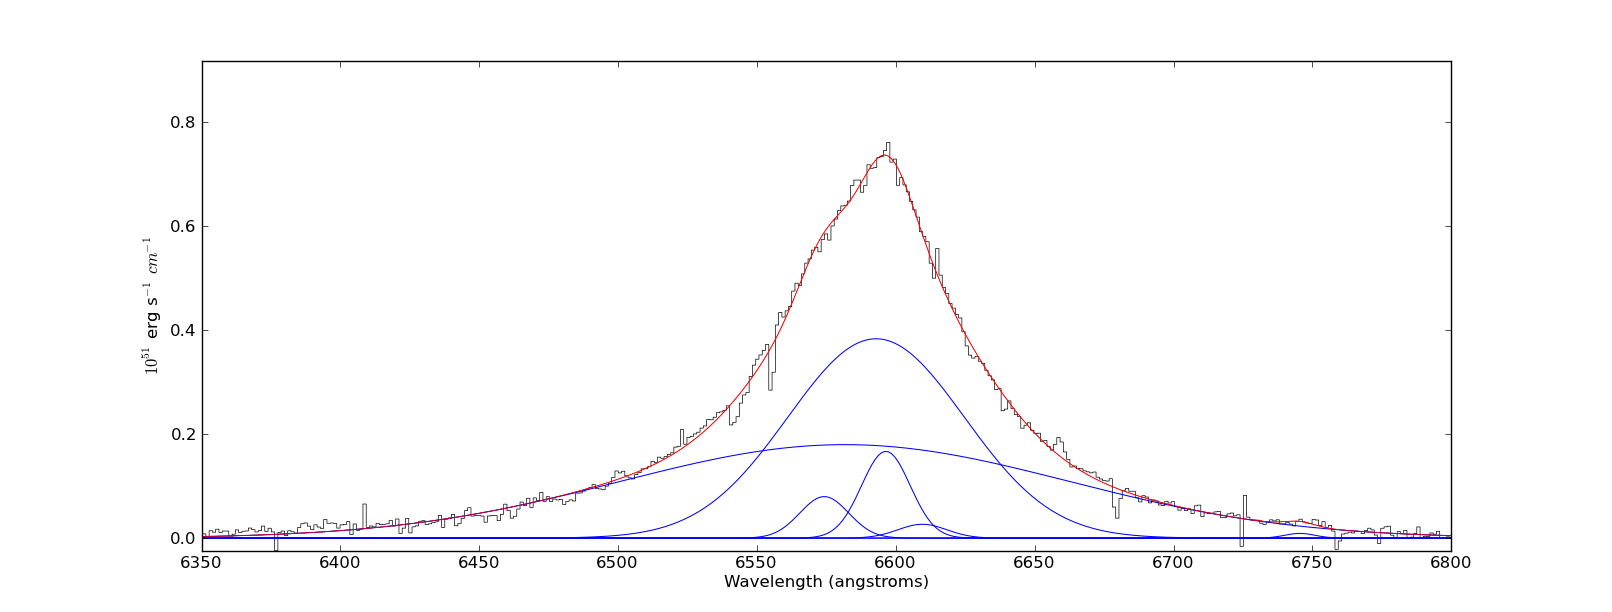
\includegraphics[width=0.46\linewidth,angle=0]{Halpha_1.png}
\vspace{5mm}
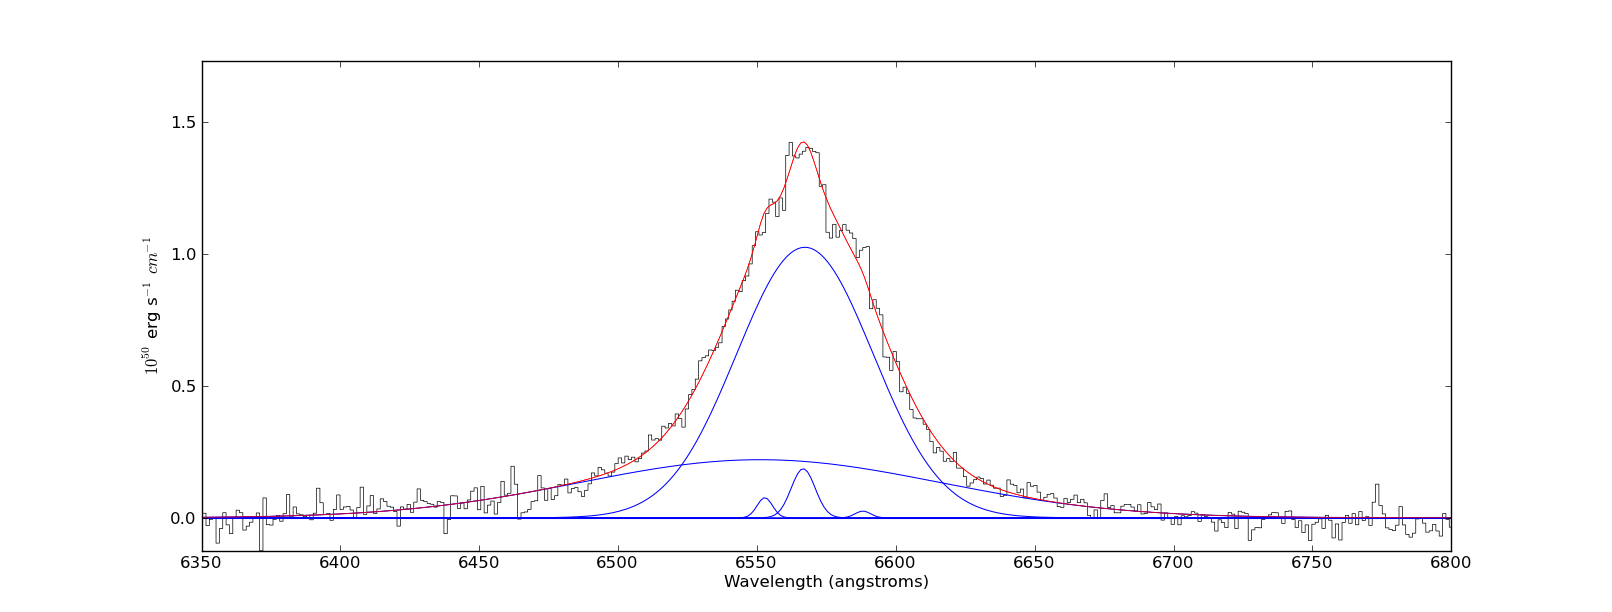
\includegraphics[width=0.49\linewidth,angle=0]{Halpha_17.png}\\
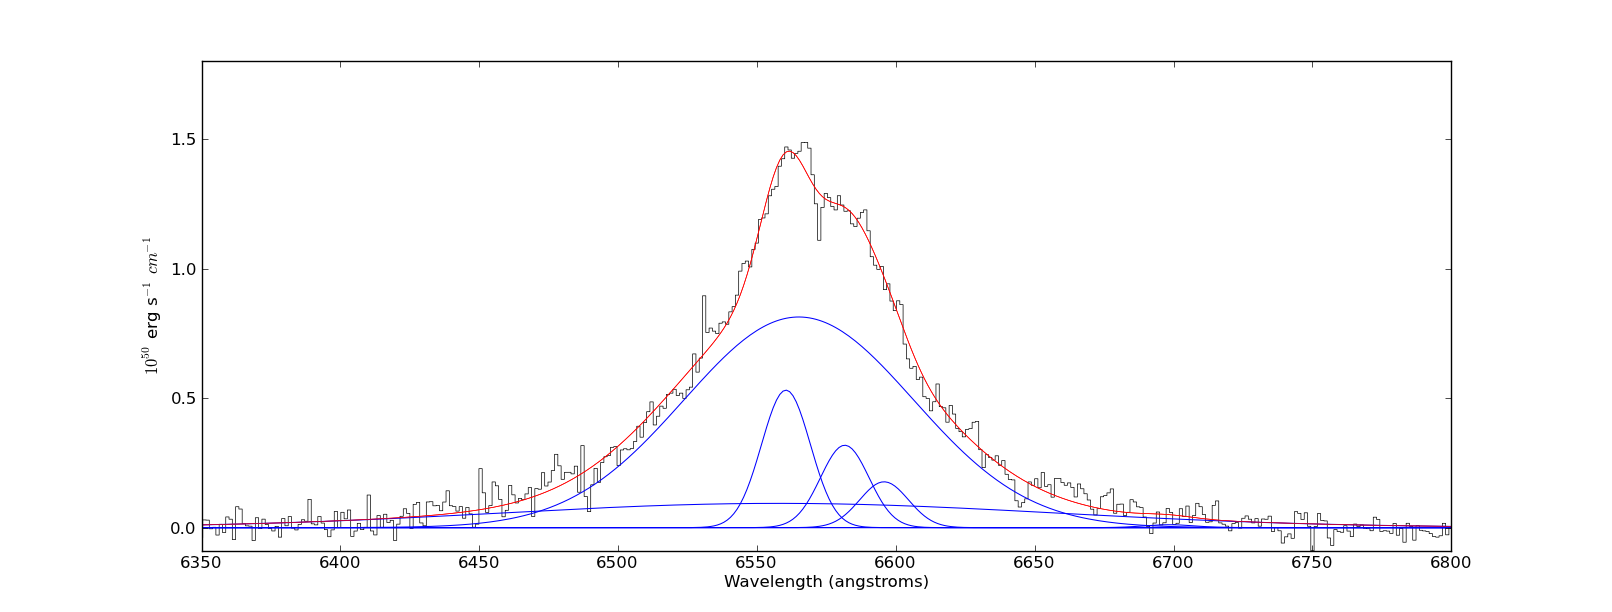
\includegraphics[width=0.46\linewidth,angle=0]{Halpha_20.png}
\end{center} 
\caption{H-$\alpha$ complex. 3500-4000A (Transitions involving  the leves from 20 until 7 (3835A) ).   top: J0155-1023 (Group A) middle: J0136-0015 (GROUP E) bottom: J0223-0007 (GROUP E) \label{fig:landscape}}   
\end{figure*}






\end{document}
